\newpage
\section*{Pruebas unitarias}
\subsection*{Smart Owl}
\begin{center}
  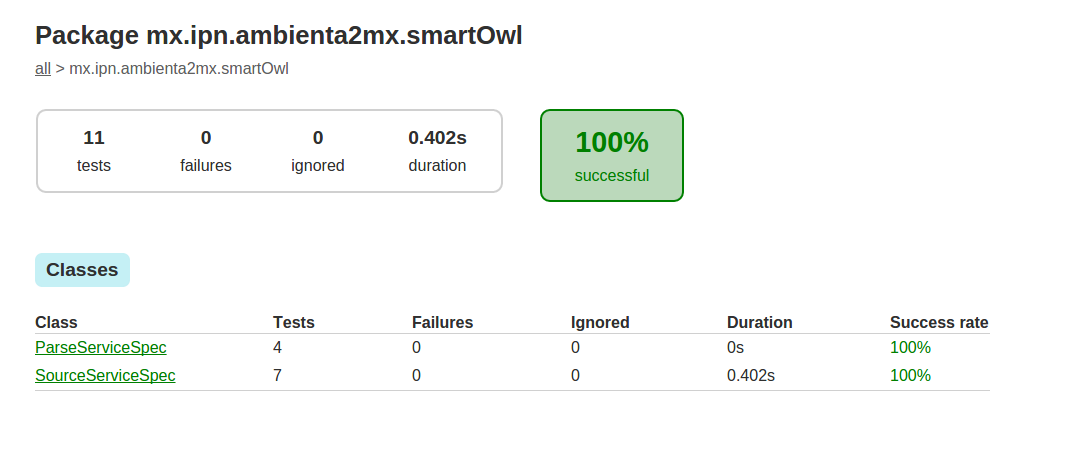
\includegraphics[width=\textwidth]{images/SmartOwlTest1}
\end{center}

\begin{center}
  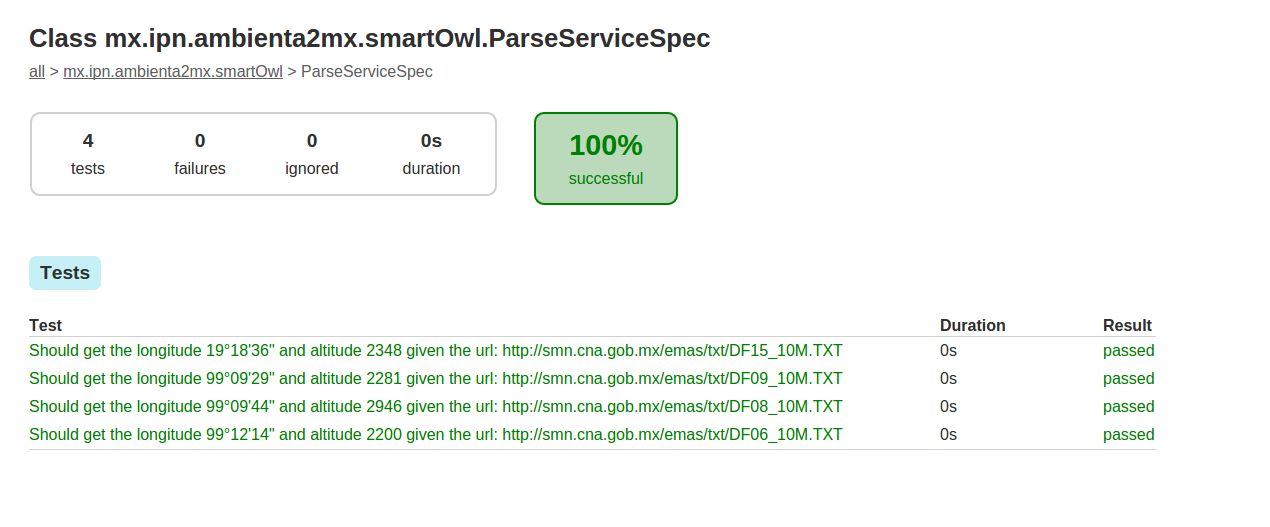
\includegraphics[width=\textwidth]{images/SmartOwlTest2}
\end{center}

\begin{center}
  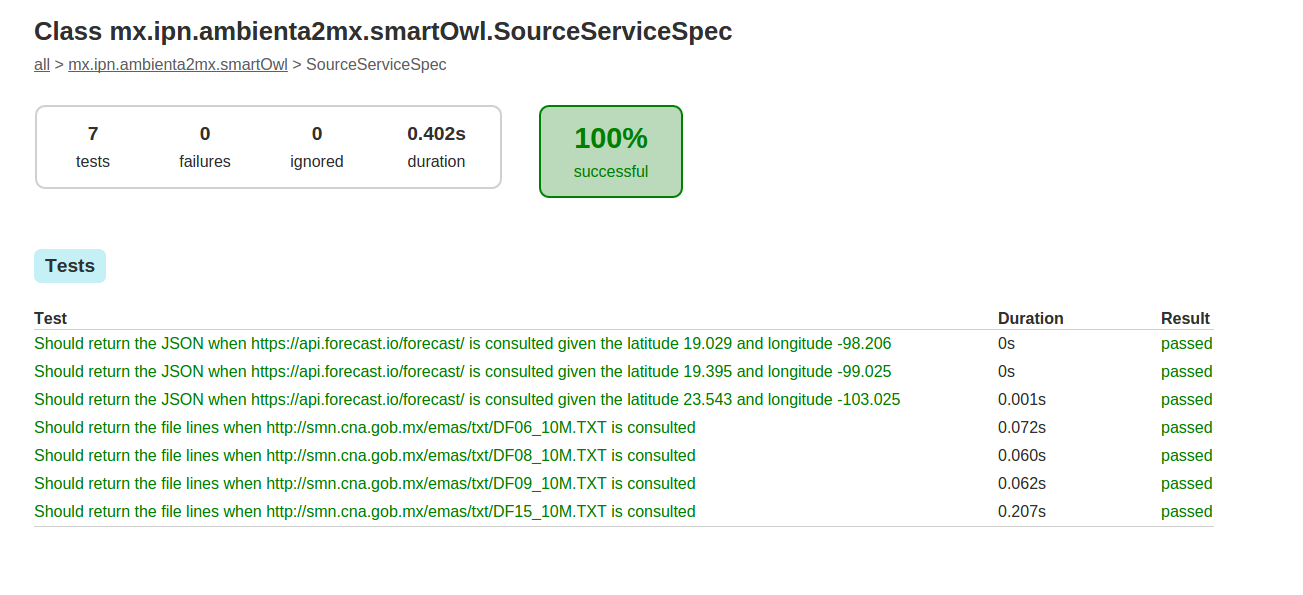
\includegraphics[width=\textwidth]{images/SmartOwlTest3}
\end{center}
\addcontentsline{toc}{chapter}{Anexo 1: Pruebas Unitarias}
%
% User stories
%
\newpage
\section*{Historias de Usuario}
\subsection*{Friendly Dolphin}
  \begin{itemize}
    \item US1 Reporte de información climática actual
    \begin{itemize}
      \item \textbf{Como} usuario de Friendly Dolphin
      \item \textbf{Quiero} consultar la información climática actual
      \item \textbf{De tal manera} que pueda generar un reporte con la información estandarizada.
    \end{itemize}
    \item Criterios de Aceptación
    \begin{itemize}
      \item Seleccionar una región del pais.
      \item Se deberá mostrar la información en texto plano.
      \item Opción para exportar la información en formato JSON o XML.
    \end{itemize}
  \end{itemize}
  \begin{itemize}
    \item US2 Historial de información climática
    \begin{itemize}
      \item \textbf{Como} usuario de Friendly Dolphin
      \item \textbf{Quiero} consultar el historial de los datos climáticos.
      \item \textbf{De tal manera} que pueda visualizar de manera gráfica el cambio de los valores de las variables climáticas a través de un periodo de tiempo
    \end{itemize}
    \item Criterios de Aceptación
    \begin{itemize}
      \item Consultar la información entre una fecha de Inicio y una fecha Final.
      \item Se deberá mostrar la información de las variables climáticas en el periodo seleccionado.
      \item Opción para exportar la información en formato JSON o XML.
    \end{itemize}
  \end{itemize}
\addcontentsline{toc}{chapter}{Anexo 2: Historias de Usuario.}